\subsubsection{Password Retreival}
			To accompany this diagram, read the Scenario \hyperref[sec:PasswordRetrievalScenario]{S.7}.

				\begin{table}[htpb]
					\centering
					\label{tab:PasswordRetrievalDiagramTable}
					\begin{tabularx}{\textwidth}{lp{9cm}}
						\hline
						\hline
							\textbf{Subject}
						& 
							\textbf{Description}\\
						\hline
							Actors	       &  Registered User, myTaxiService Web Application, myTaxiService Server\\
						\hline
							Preconditions  &  Registered User must be actually registered.\\
						\hline
							Execution      &  1.~Registered User opens the myTaxiService Web Application.\\
										   &  2.~Registered User taps on the "Retrieve Password" link.\\
										   &  3.~myTaxiService Web Application shows the email field.\\
										   &  4.~Registered User inserts his email.\\
										   &  5.~Registered User taps on the "Retrieve" button.\\
										   &  6.~myTaxiService Web Application calls the password retrieval function.\\
										   &  7.~myTaxiService Server verifies the email.\\
										   &  8.~myTaxiService Server replies with an ok or an error\\
										   &  9.~myTaxiService Web Application shows to the Registered User the result.\\
						\hline
							Postconditions &  The system has sent an email to the Registered User containing his password.\\
						\hline
							Exceptions     &  1.~The Registered User disconnects before clicking on the "Retrieve" button.\\
									
						\hline
						\hline
					\end{tabularx}
				\end{table}
				
				\begin{figure}[H]
					\centering
					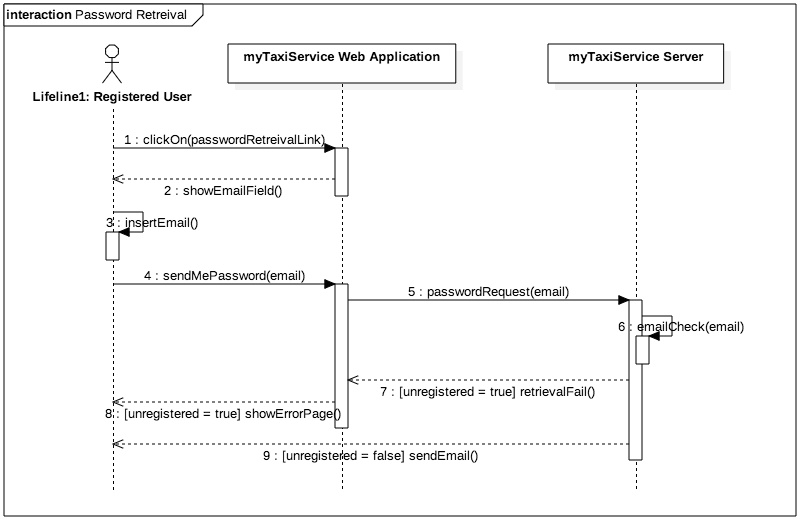
\includegraphics[width=\textwidth, scale=0.5]{IMG/InteractionDiagrams/PasswordRetrieval.png}
					\caption{Password Retrieval Interaction Diagram}\label{sec:FigureProfileModification}
				\end{figure}